% Canonical survey figures. Inputted where referenced.

% ---------------------------------------------------------------------------
% Opening figure: conceptual evolution tree for the survey thesis.
% ---------------------------------------------------------------------------
\newcommand{\figevolution}{%
\begin{figure}[t]
\centering
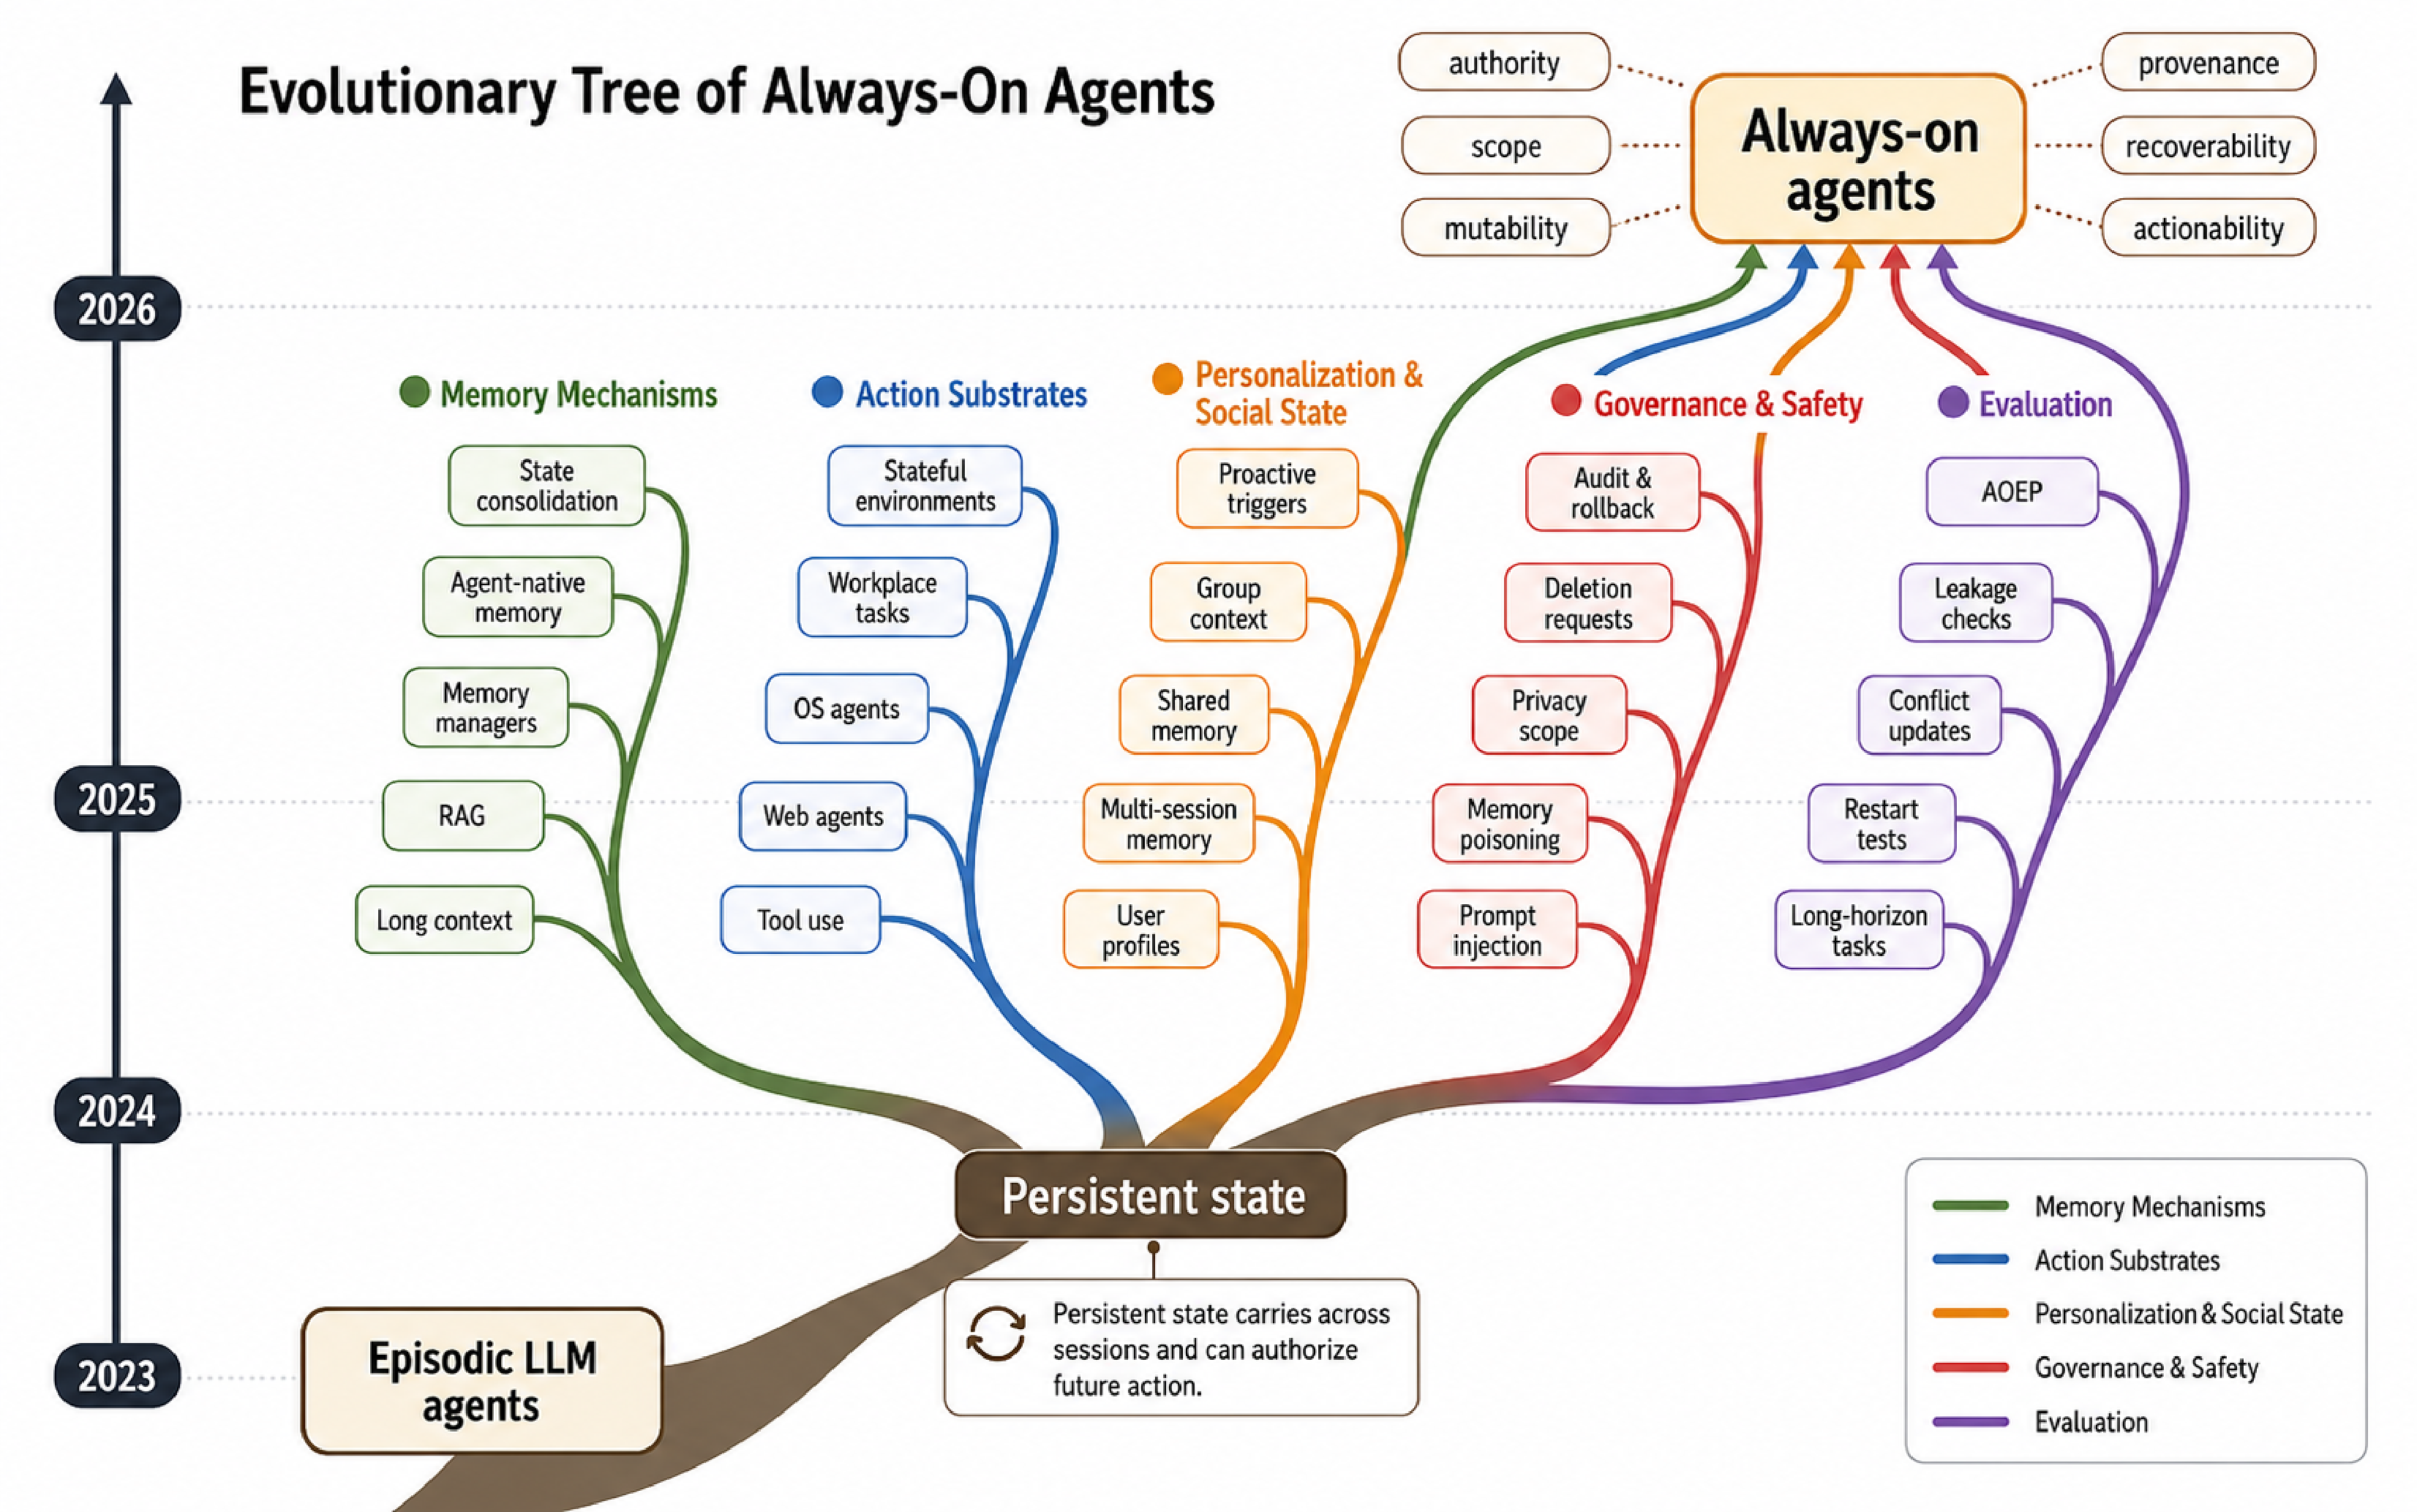
\includegraphics[width=\linewidth]{figures_always_on_agents_evolution_tree.pdf}
\caption{Evolutionary tree of always-on agents. The figure sketches the survey's
organizing claim: episodic LLM agents become always-on not by running
continuously, but when durable state persists across sessions and can authorize
future action. Five strands map the field's current build-out: memory mechanisms,
action substrates, personalization and social state, governance and safety, and
evaluation. The target state is qualified by six diagnostic axes: authority,
scope, mutability, provenance, recoverability, and actionability. These are the
questions that make persistence governable rather than only useful.}
\label{fig:evolution-tree}
\end{figure}}

% ---------------------------------------------------------------------------
% FIGURE 1: Overview stack -- the Substance / Motion / Control organization.
% ---------------------------------------------------------------------------
\newcommand{\figoverview}{%
\begin{figure}[t]
\centering
\resizebox{\linewidth}{!}{%
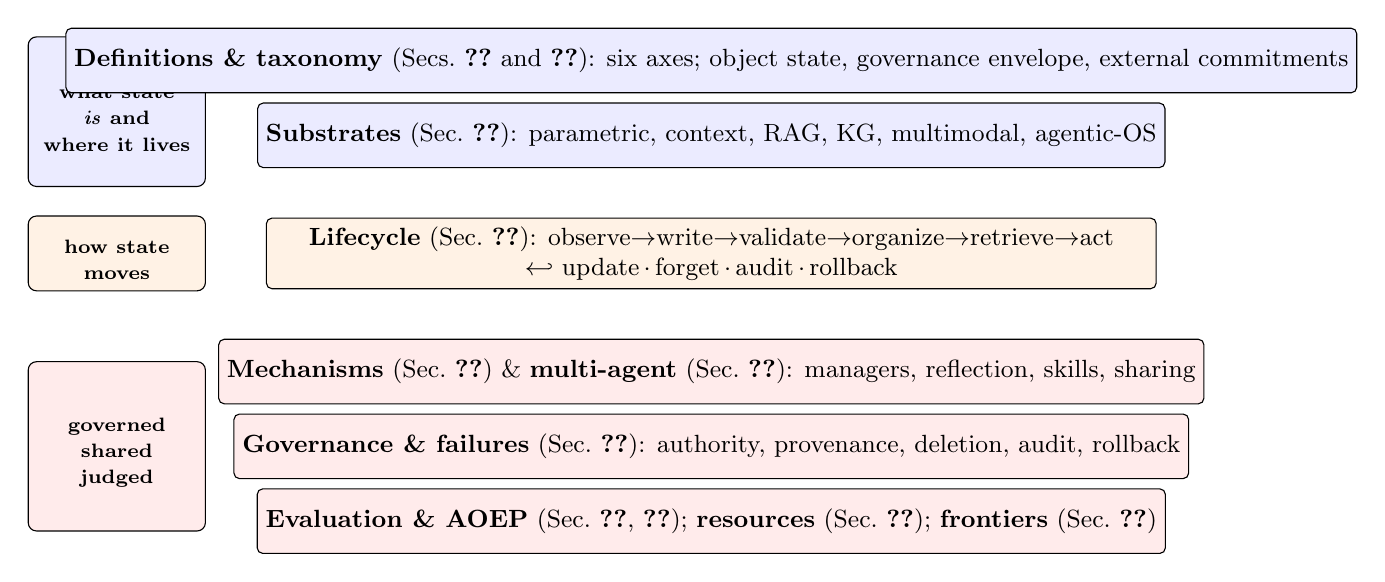
\begin{tikzpicture}[font=\small,
  layer/.style={draw,rounded corners=2pt,minimum width=11.3cm,minimum height=0.82cm,align=center,inner sep=3pt},
  regime/.style={draw,rounded corners=3pt,minimum width=2.25cm,align=center,font=\footnotesize\bfseries,inner sep=4pt},
  lens/.style={draw,dashed,rounded corners=2pt,minimum width=3.5cm,minimum height=0.7cm,align=center,font=\footnotesize}]
% the regime column (left)
\node[regime,fill=blue!8,minimum height=1.9cm] (sub) at (-7.45,2.35) {\substance\\\scriptsize what state\\\scriptsize \emph{is} and\\\scriptsize where it lives};
\node[regime,fill=orange!10,minimum height=0.95cm] (mot) at (-7.45,0.55) {\motion\\\scriptsize how state\\\scriptsize moves};
\node[regime,fill=red!8,minimum height=2.15cm] (con) at (-7.45,-1.9) {\control\\\scriptsize governed\\\scriptsize shared\\\scriptsize judged};
% the layers (right), stacked
\node[layer,fill=blue!8] (l1) at (0.1,3.0) {\textbf{Definitions \& taxonomy} (Secs.~\ref{sec:definition} and~\ref{sec:statetax}): six axes; object state, governance envelope, external commitments};
\node[layer,fill=blue!8] (l2) at (0.1,2.05) {\textbf{Substrates} (Sec.~\ref{sec:substrates}): parametric, context, RAG, KG, multimodal, agentic-OS};
\node[layer,fill=orange!10] (l3) at (0.1,0.55) {\textbf{Lifecycle} (Sec.~\ref{sec:lifecycle}): observe$\to$write$\to$validate$\to$organize$\to$retrieve$\to$act\\$\hookleftarrow$ update$\,\cdot\,$forget$\,\cdot\,$audit$\,\cdot\,$rollback};
\node[layer,fill=red!8] (l4) at (0.1,-0.95) {\textbf{Mechanisms} (Sec.~\ref{sec:mechanisms}) \& \textbf{multi-agent} (Sec.~\ref{sec:mechanisms}): managers, reflection, skills, sharing};
\node[layer,fill=red!8] (l5) at (0.1,-1.9) {\textbf{Governance \& failures} (Sec.~\ref{sec:failures}): authority, provenance, deletion, audit, rollback};
\node[layer,fill=red!8] (l6) at (0.1,-2.85) {\textbf{Evaluation \& AOEP} (Sec.~\ref{sec:evaluation},~\ref{sec:aoep}); \textbf{resources} (Sec.~\ref{sec:resources}); \textbf{frontiers} (Sec.~\ref{sec:frontiers})};
\end{tikzpicture}}
\caption{The survey is organized as a three-regime stack. \substance{} asks what
persistent state \emph{is} and where it physically lives; \motion{} asks how state
moves through the agent's operating loop; \control{} asks how that movement is
governed, shared, and judged. In our coding, work is concentrated more heavily on
accumulating and retrieving state than on governing, recovering, or relinquishing it.}
\label{fig:overview}
\end{figure}}

% ---------------------------------------------------------------------------
% FIGURE 2: Corpus coverage heatmap -- lifecycle stage x taxonomy part.
% Values are counts of works in each part whose coding touches each stage.
% The visual point: the return arc (forget/audit/rollback) is pale everywhere.
% ---------------------------------------------------------------------------
\newcommand{\figheatmap}{%
\begin{figure}[t]
\centering
\resizebox{\linewidth}{!}{%
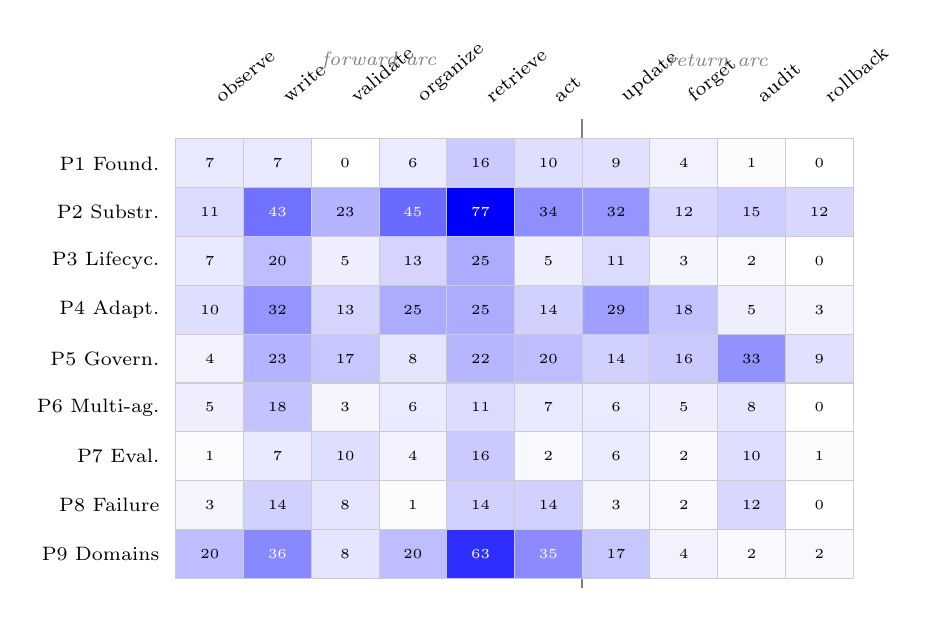
\begin{tikzpicture}[font=\scriptsize,x=0.86cm,y=0.62cm]
% data: rows = parts P1..P9, cols = 10 stages. max for color scale = 77.
\def\stages{observe,write,validate,organize,retrieve,act,update,forget,audit,rollback}
\foreach \lab/\j in {observe/0,write/1,validate/2,organize/3,retrieve/4,act/5,update/6,forget/7,audit/8,rollback/9}{
  \node[rotate=40,anchor=west,font=\scriptsize] at (\j+0.5,9.7) {\lab};}
% return-arc separator
\draw[thick,gray] (6,-0.2) -- (6,9.4);
\node[font=\scriptsize\itshape,gray] at (8,10.6) {return arc};
\node[font=\scriptsize\itshape,gray] at (3,10.6) {forward arc};
\foreach \p/\i/\name in {P1/8/{P1 Found.},P2/7/{P2 Substr.},P3/6/{P3 Lifecyc.},P4/5/{P4 Adapt.},P5/4/{P5 Govern.},P6/3/{P6 Multi-ag.},P7/2/{P7 Eval.},P8/1/{P8 Failure},P9/0/{P9 Domains}}{
  \node[anchor=east,font=\scriptsize] at (-0.1,\i+0.5) {\name};}
% cell macro: \cell{col}{row}{value}; color intensity = value/77
\foreach \i/\row in {%
  8/{7,7,0,6,16,10,9,4,1,0},
  7/{11,43,23,45,77,34,32,12,15,12},
  6/{7,20,5,13,25,5,11,3,2,0},
  5/{10,32,13,25,25,14,29,18,5,3},
  4/{4,23,17,8,22,20,14,16,33,9},
  3/{5,18,3,6,11,7,6,5,8,0},
  2/{1,7,10,4,16,2,6,2,10,1},
  1/{3,14,8,1,14,14,3,2,12,0},
  0/{20,36,8,20,63,35,17,4,2,2}}{
  \foreach \v [count=\j from 0] in \row {
    \pgfmathsetmacro\shade{min(100,\v/77*100)}
    \fill[blue!\shade!white,draw=gray!40] (\j,\i) rectangle (\j+1,\i+1);
    \pgfmathsetmacro\txtcol{\v>40?1:0}
    \node[font=\tiny,text=\ifdim\shade pt>45pt white\else black\fi] at (\j+0.5,\i+0.5) {\v};}}
\end{tikzpicture}}
\caption{Coverage heatmap: for each taxonomy part (rows), the number of coded works
whose lifecycle coding touches each stage (columns). Cells are shaded by count.
The forward arc (left of the divider) is dark across nearly every part; the return
arc, especially \texttt{forget}, \texttt{audit}, and \texttt{rollback}, stays pale
even in the governance part (P5). This is the survey's main asymmetry made
visual. Counts are per-part stage incidences and exceed part sizes because coding is
multi-label.}
\label{fig:heatmap}
\end{figure}}

% ---------------------------------------------------------------------------
% FIGURE 3: The lifecycle arc -- forward and return, with invariants.
% ---------------------------------------------------------------------------
\newcommand{\figlifecycle}{%
\begin{figure}[t]
\centering
\resizebox{\linewidth}{!}{%
\begin{tikzpicture}[font=\footnotesize,
  st/.style={draw,rounded corners=2pt,minimum height=0.7cm,minimum width=1.35cm,align=center,inner sep=2pt},
  fwd/.style={st,fill=orange!12}, ret/.style={st,fill=red!10},
  ar/.style={-{Stealth[length=2mm]},thick}]
% forward arc (left to right, top)
\node[fwd] (obs) at (0,2) {observe};
\node[fwd] (wr) at (1.75,2) {write};
\node[fwd] (val) at (3.5,2) {validate};
\node[fwd] (org) at (5.25,2) {organize};
\node[fwd] (ret) at (7.0,2) {retrieve};
\node[fwd] (act) at (8.75,2) {act};
\draw[ar] (obs)--(wr); \draw[ar] (wr)--(val); \draw[ar] (val)--(org); \draw[ar] (org)--(ret); \draw[ar] (ret)--(act);
% return arc (right to left, bottom)
\node[ret] (upd) at (8.75,0) {update};
\node[ret] (frg) at (7.0,0) {forget};
\node[ret] (aud) at (5.25,0) {audit};
\node[ret] (rb) at (3.5,0) {rollback};
\draw[ar] (act)--(upd); \draw[ar] (upd)--(frg); \draw[ar] (frg)--(aud); \draw[ar] (aud)--(rb);
\draw[ar,dashed] (rb) to[out=180,in=180] (obs);
\node[font=\scriptsize\itshape,orange!60!black] at (4.4,2.7) {forward arc: accumulate \& use (well-served)};
\node[font=\scriptsize\itshape,red!60!black] at (6.1,-0.7) {return arc: govern \& recover (sparse: rollback 27/435)};
% invariants band
\node[draw,dashed,rounded corners,fill=gray!6,minimum width=10.5cm,align=center,font=\scriptsize] at (4.4,-1.7)
  {\textbf{Five invariants} the loop should preserve: authority monotonicity~$\cdot$~scope non-expansion~$\cdot$~deletion propagation~$\cdot$~provenance preservation~$\cdot$~rollback traceability};
\end{tikzpicture}}
\caption{The persistent-state lifecycle. State flows along a forward arc that
accumulates and uses it, then a return arc that updates, forgets, audits, and rolls
it back once outcomes are known. The forward arc is heavily studied; the return arc
is sparse (only $27$ of $435$ corpus works expose any rollback mechanism). Five
invariants should hold across the whole loop; each failure mode in
Section~\ref{sec:failures} violates one of them.}
\label{fig:lifecycle}
\end{figure}}

% ---------------------------------------------------------------------------
% FIGURE 4: AOEP evaluation flow.
% ---------------------------------------------------------------------------
\newcommand{\figaoep}{%
\begin{figure}[t]
\centering
\resizebox{\linewidth}{!}{%
\begin{tikzpicture}[font=\footnotesize,
  bx/.style={draw,rounded corners=2pt,align=center,minimum height=0.85cm,inner sep=3pt},
  ar/.style={-{Stealth[length=2mm]},thick}]
\node[bx,fill=blue!8] (ep) at (0,0) {Episode:\\event stream\\(typed ops)};
\node[bx,fill=blue!8] (san) at (2.6,0) {Sanitize:\\strip oracle\\fields};
\node[bx,fill=orange!10] (sys) at (5.3,0) {System under\\test maintains\\its own state};
\node[bx,fill=orange!10] (prb) at (8.0,0) {Neutral\\probes\\(IDs only)};
\node[bx,fill=red!8] (val) at (10.7,0) {Validator:\\compute invariants,\\score vs oracle};
\draw[ar] (ep)--(san); \draw[ar] (san)--(sys); \draw[ar] (sys)--(prb); \draw[ar] (prb)--(val);
\node[bx,fill=red!8,minimum width=10cm,align=center] (out) at (5.3,-1.6)
  {\textbf{Deterministic scorecard:} obligation pass (must actively satisfy) vs negative-invariant pass (no-leakage, satisfiable by storing nothing)};
\draw[ar] (val) to[out=270,in=0] (out.east);
\end{tikzpicture}}
\caption{The Always-On Evaluation Protocol (AOEP). Each episode is a typed event
stream; outcome-revealing fields are stripped before a system under test consumes it;
the system answers neutral probes; a validator recomputes the invariants itself and
scores against an oracle. Obligation pass (positive duties a system must actively
meet) is reported separately from negative-invariant pass (no-leakage checks, which a
system that stores nothing satisfies vacuously), so recall and governance are scored
on different axes.}
\label{fig:aoep}
\end{figure}}

% ---------------------------------------------------------------------------
% FIGURE 5: Stage-proxy invariant opportunity heatmap. This is not direct
% invariant enforcement: a work counts toward an invariant if it touches the
% lifecycle stage(s) where that invariant would be established or checked.
% Color scale max = 92.
% ---------------------------------------------------------------------------
\newcommand{\figinvariants}{%
\begin{figure}[t]
\centering
\resizebox{0.92\linewidth}{!}{%
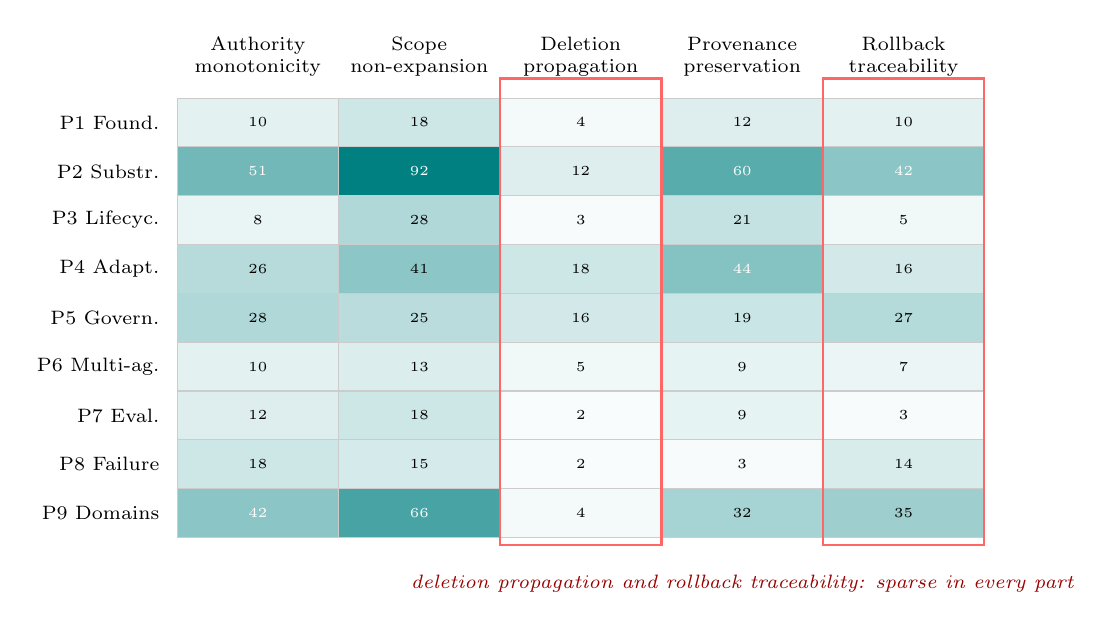
\begin{tikzpicture}[font=\scriptsize,x=2.05cm,y=0.62cm]
\foreach \lab/\j in {{Authority\\monotonicity}/0,{Scope\\non-expansion}/1,{Deletion\\propagation}/2,{Provenance\\preservation}/3,{Rollback\\traceability}/4}{
  \node[align=center,font=\scriptsize] at (\j+0.5,9.85) {\lab};}
\foreach \p/\i in {{P1 Found.}/8,{P2 Substr.}/7,{P3 Lifecyc.}/6,{P4 Adapt.}/5,{P5 Govern.}/4,{P6 Multi-ag.}/3,{P7 Eval.}/2,{P8 Failure}/1,{P9 Domains}/0}{
  \node[anchor=east,font=\scriptsize] at (-0.05,\i+0.5) {\p};}
\foreach \i/\row in {%
  8/{10,18,4,12,10},
  7/{51,92,12,60,42},
  6/{8,28,3,21,5},
  5/{26,41,18,44,16},
  4/{28,25,16,19,27},
  3/{10,13,5,9,7},
  2/{12,18,2,9,3},
  1/{18,15,2,3,14},
  0/{42,66,4,32,35}}{
  \foreach \v [count=\j from 0] in \row {
    \pgfmathsetmacro\shade{min(100,\v/92*100)}
    \fill[teal!\shade!white,draw=gray!40] (\j,\i) rectangle (\j+1,\i+1);
    \node[font=\tiny,text=\ifdim\shade pt>45pt white\else black\fi] at (\j+0.5,\i+0.5) {\v};}}
% mark the two structurally sparse invariants
\draw[thick,red!60] (2,-0.15) rectangle (3,9.4);
\draw[thick,red!60] (4,-0.15) rectangle (5,9.4);
\node[font=\scriptsize\itshape,red!60!black,align=center] at (3.5,-0.95) {deletion propagation and rollback traceability: sparse in every part};
\end{tikzpicture}}
\caption{Stage-proxy opportunity for the five invariants, by taxonomy part. A work
counts toward an invariant if its lifecycle coding touches the stage that would
establish or check that
invariant (authority monotonicity at validate/act; scope non-expansion at
organize/retrieve; deletion propagation at forget; provenance preservation at
organize/update; rollback traceability at act/rollback), shaded by count. The
two boxed columns, deletion propagation and rollback traceability, are pale in
every part including the governance part (P5): the two invariants that most
distinguish a governed persistent-state system have few stage opportunities in
the coded corpus. This figure should not be read as direct evidence that a paper
tested or enforced an invariant; it is a proxy view of where the relevant
lifecycle stages appear.}
\label{fig:invariants}
\end{figure}}

% ---------------------------------------------------------------------------
% FIGURE 6: Corpus timeline. Share of each year's works touching early vs
% governance vs rollback stages, 2023-2026. Shows the gap is recent and thin.
% ---------------------------------------------------------------------------
\newcommand{\figtimeline}{%
\begin{figure}[t]
\centering
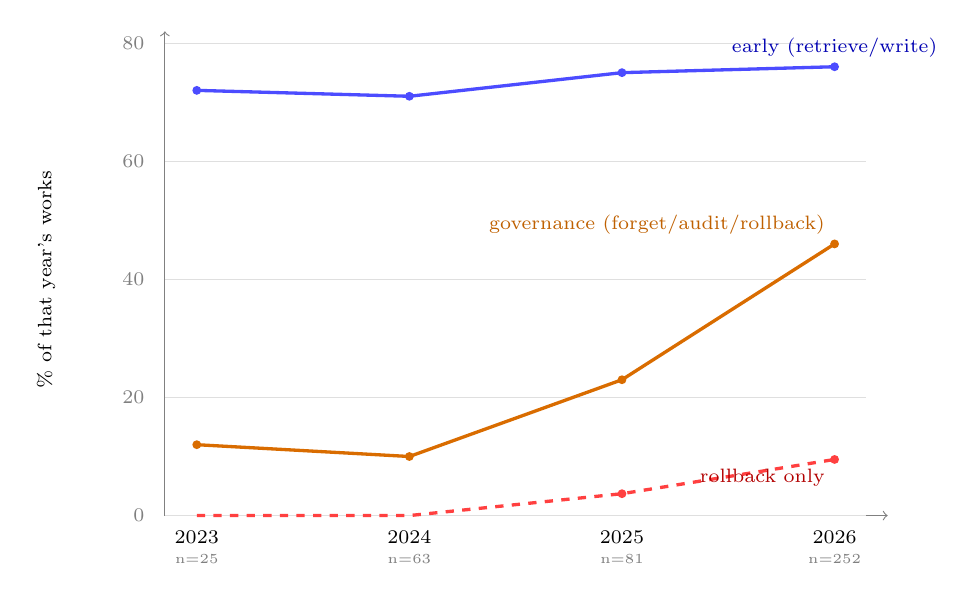
\begin{tikzpicture}[font=\small,x=2.7cm,y=0.075cm]
% axes
\draw[->,gray] (-0.15,0) -- (3.25,0);
\draw[->,gray] (-0.15,0) -- (-0.15,82);
\foreach \yv in {0,20,40,60,80}{ \node[anchor=east,font=\scriptsize,gray] at (-0.2,\yv) {\yv}; \draw[gray!25] (-0.15,\yv)--(3.15,\yv);}
\node[rotate=90,anchor=south,font=\scriptsize] at (-0.62,40) {\% of that year's works};
\foreach \x/\lab/\n in {0/2023/25,1/2024/63,2/2025/81,3/2026/252}{ \node[anchor=north,font=\scriptsize] at (\x,-1) {\lab}; \node[anchor=north,font=\tiny,gray] at (\x,-5) {n=\n};}
% early (retrieve/write): 72,71,75,76 -- flat high (blue)
\draw[blue!70,very thick] (0,72)--(1,71)--(2,75)--(3,76);
\foreach \x/\y in {0/72,1/71,2/75,3/76}{\fill[blue!70](\x,\y)circle(1.6pt);}
\node[blue!70!black,font=\scriptsize,anchor=south] at (3,76) {early (retrieve/write)};
% governance (forget/audit/rollback): 12,10,23,46 (orange)
\draw[orange!85!black,very thick] (0,12)--(1,10)--(2,23)--(3,46);
\foreach \x/\y in {0/12,1/10,2/23,3/46}{\fill[orange!85!black](\x,\y)circle(1.6pt);}
\node[orange!75!black,font=\scriptsize,anchor=south east] at (3,46) {governance (forget/audit/rollback)};
% rollback only: 0,0,3.7,9.5 (red, dashed)
\draw[red!75,very thick,dashed] (0,0)--(1,0)--(2,3.7)--(3,9.5);
\foreach \x/\y in {2/3.7,3/9.5}{\fill[red!75](\x,\y)circle(1.6pt);}
\node[red!70!black,font=\scriptsize,anchor=north east] at (3,9.5) {rollback only};
\end{tikzpicture}
\caption{Corpus coverage over time, as the share of each year's coded works whose
lifecycle touches an early stage (retrieve or write), any governance stage (forget,
audit, or rollback), or rollback specifically. Early-stage coverage is flat and high
across the period; governance coverage rises from $12\%$ to $46\%$ but remains a
minority, and rollback rises only from $0\%$ to under $10\%$. In the works we
coded, the governance turn is recent (it begins in earnest only in 2025) and still
thin. Per-year corpus sizes are shown on the axis and sum to $421$ because the
fourteen pre-2023 foundational anchors are excluded from this year-by-year view.
The count for 2026 is necessarily incomplete and preprint-heavy, as discussed in
Section~\ref{sec:frontiers}.}
\label{fig:timeline}
\end{figure}}
